\newcommand{\bfvec}[1]{%
    \mathbf{#1}
    }
\newcommand{\filtuvec}{%
    \mathbf{\tilde{u}}
    }
\newcommand{\filtsvec}{%
    \mathbf{\tilde{S}}
    }
\newcommand{\filtwvec}{%
    \mathbf{\tilde{\omega}}
    }
\newcommand{\filterns}{%
    \pdv{\filtuvec}{t} + \mathbf{\tilde{u}} \cdot \grad{\mathbf{\tilde{u}}} = 
        -\grad{p} + \nu \laplacian{\mathbf{\tilde{u}}} - \div \mathbf{\tau}
    }
\section{Filtered Enstrophy Equation}
To derive the filtered enstrophy equation we start by determining the
filtered vorticity equation from the filtered Navier-Stokes equations,
\begin{subequations}
    \begin{equation}
        \div \filtuvec = 0
        \label{eq:filtered-mass}
    \end{equation}
    \begin{equation}
        \filterns
        \label{eq:filtered-momentum}
    \end{equation}
\end{subequations}

The transport equation for vorticity, $\mathbf{\tilde{\omega}} \equiv \curl
\filtuvec $, can be obtained by taking the curl of the above equation. 
Applying the curl to Eq.~\ref{eq:filtered-momentum} gives
\begin{subequations}
    \begin{equation}
        \curl \left(\filterns\right)
    \end{equation}
    \begin{equation}
        \pdv{\filtwvec}{t} + \filtuvec \cdot \grad \filtwvec =
            \filtwvec \cdot \grad \filtuvec + \nu \laplacian{\filtwvec}
            - \curl \div \mathbf{\tau}
    \end{equation}
    \label{eq:filtered-vorticity}
\end{subequations}

Note in deriving Eq.~\ref{eq:filtered-vorticity} we have applied the following vector
identities
\begin{subequations}
    \begin{equation}
        \bfvec{u} \cdot \grad \bfvec{u} = 
                \grad\left(\frac{1}{2}\bfvec{u} \cdot \bfvec{u}\right) 
                - \bfvec{u} \cp \left(\curl \bfvec{u}\right)
    \end{equation}
    \begin{equation}
        \curl \grad \phi = 0
    \end{equation}
    \begin{equation}
        \div \curl \mathbf{a} = 0
    \end{equation}
\end{subequations}

Next we can multiply Eq.~\ref{eq:filtered-vorticity} to obtain the filtered
enstrophy, $\Omega \equiv \frac{1}{2} \filtwvec \filtwvec$, transport
equation, namely,
\begin{subequations}
    \begin{equation}
        \filtwvec \cdot \bigg(
        \pdv{\filtwvec}{t} + \filtuvec \cdot \grad \filtwvec =
            \filtwvec \cdot \grad \filtuvec + \nu \laplacian{\filtwvec}
            - \curl \div \mathbf{\tau}
            \bigg)
    \end{equation}
    \begin{equation}
        \pdv{\Omega}{t} + \filtuvec \cdot \grad \Omega = 
            \filtwvec \cdot \filtsvec \cdot \filtwvec + \nu \laplacian{\Omega}
            - \nu \grad \filtwvec : \grad \filtwvec 
            - \filtwvec \cdot \curl \div \mathbf{\tau}
            \label{eq:enstrophy-vector}
    \end{equation}
\end{subequations}


\subsection{Subgrid Stress Enstrophy Evaluation}
As we shall see, it is helpful to evaluate transport equations in terms of
their physical representation (e.g., transport, dissipation, and
production). In the following we will separate the subgrid stress term into
both transport and production terms in order to obtain physical insight.
We begin the evaluation by expressing the subgrid stress in index notation,
\begin{equation}
    -\filtwvec \cdot \curl \div \tau =
        - \varepsilon_{ijk} \tilde{\omega}_{i} 
        \pdv{}{x_{j}} \pdv{}{x_{l}} \tau_{kl}
\end{equation}
Interchanging the linear derivative operators and moving the Levi-Civita
inside the first derivative gives
\begin{equation}
        - \varepsilon_{ijk} \tilde{\omega}_{i}  \pdv{}{x_{j}} \pdv{}{x_{l}}
        \tau_{kl} =
        - \tilde{\omega}_{i}  \pdv{}{x_{l}} \underbrace{\varepsilon_{ijk} \pdv{}{x_{j}}
        \tau_{kl}}_{\equiv \curl \mathbf{\tau}}
\end{equation}
Substituting in $\Psi_{il}$ for $\curl \mathbf{\tau}$ the following can be 
arranged to get 
\begin{equation}
    \begin{split}
        - \tilde{\omega}_{i}  \pdv{}{x_{l}} \varepsilon_{ijk} \pdv{}{x_{j}} \tau_{kl}  = &
            -\tilde{\omega}_{i} \pdv{\Psi_{il}}{x_{l}} \\
            & = - \underbrace{\pdv{}{x_{l}}\big(\tilde{\omega}_{i} \Psi_{il} \big)}_{\equiv \text{Transport}}
            + \underbrace{\Psi_{il} \pdv{\tilde{\omega}_{i}}{x_{l}}}_{\equiv \text{Production}}
    \end{split}
    \label{eq:trans-enstrophy}
\end{equation}
Therefore from Eq.~\ref{eq:trans-enstrophy} it is clear that that the transport
of enstrophy from the subgrid stress is due to 
\begin{equation}
    \colorboxed{red}{
        - \pdv{}{x_{l}}\big(\tilde{\omega}_{i} \Psi_{il} \big)
    }
    \label{eq:SGS-enstrophy-transport}
\end{equation}
while the production of enstrophy from SGS $P_{\Omega}$ is given by
\begin{equation}
    \colorboxed{red}{
        P_{\Omega} \equiv  \Psi_{il} \pdv{\tilde{\omega}_{i}}{x_{l}}  =
            \varepsilon_{ijk} \pdv{\widetilde{\omega}_{i}}{x_{l}}
            \pdv{\tau_{kl}}{x_{j}}
            \label{eq:SGS-enstrophy-production}
    }
\end{equation}
Similarly to the above analysis of the kinetic production, we will next 
systematically evaluate the enstrophy production using the SGS given in
Eq.~\ref{eq:SGS-tf-8} 
\input{latex-inputs/c2-enstrophy-production-2}
\newcommand{\pienst}{\Pi_{\Omega}}
\newcommand{\penst}{P_{\Omega}}
\newcommand{\aenst}{A_{\Omega}}
\newcommand{\benst}{B_{\Omega}}
\newcommand{\denst}{D_{\Omega}}
\newcommand{\matderv}[1]{\frac{D#1}{Dt}}

\subsection{Term-by-Term Enstrophy Transport Evaluation}
To understand the blowup and healing process of the energetics it makes sense to examine the
transport equation for the filtered enstrophy. We start by substituting in
Eqs.~\ref{eq:SGS-enstrophy-production} \& \ref{eq:SGS-enstrophy-transport} into
Eq.~\ref{eq:enstrophy-vector} to get the following in index notation
\begin{equation}
    \underbrace{\pdv{\Omega}{t} + \widetilde{u}_{j} \pdv{\Omega}{x_{i}}}_{\equiv \matderv{\Omega}} =
        \underbrace{\widetilde{\omega}_{i} \widetilde{S}_{ij} \widetilde{\omega}_{j}}_{\equiv A_{\Omega}}
        \underbrace{+ \nu \pdv{}{x_{j}} \left( \pdv{\Omega}{x_{j}} \right)}_{\equiv B_{\Omega}}
        \underbrace{- \nu \pdv{\widetilde{\omega_{i}}}{x_{j}}\pdv{\widetilde{\omega}_{i}}{x_{j}}}_{\equiv D_{\Omega}}
        \underbrace{- \pdv{}{x_{j}} \left(\widetilde{\omega} \Psi_{il}\right)}_{\equiv \Pi_{\Omega}} 
        \underbrace{+ \Psi_{il} \pdv{\widetilde{\omega}_{i}}{x_{j}}}_{\equiv P_{\Omega}} 
        \label{eq:enstrophy-transport}
\end{equation}
where we can define the following budget terms as
\begin{subequations}
    \begin{align}
        A_{\Omega} \equiv \; &
            \widetilde{\omega}_{i} \widetilde{S}_{ij} \widetilde{\omega}_{j}\\
        B_{\Omega} \equiv \; &
            \nu \pdv{}{x_{j}} \left( \pdv{\Omega}{x_{j}} \right)\\
        D_{\Omega} \equiv \; &
            -\nu \pdv{\widetilde{\omega_{i}}}{x_{j}}\pdv{\widetilde{\omega}_{i}}{x_{j}}\\
        \Pi_{\Omega} \equiv \; &
            -\pdv{}{x_{j}} \left(\widetilde{\omega} \Psi_{il}\right)\\
        P_{\Omega} \equiv \; &
            \Psi_{il} \pdv{\widetilde{\omega}_{i}}{x_{j}}
    \end{align}
\end{subequations}

On the right side of Eq.~\ref{eq:enstrophy-transport}
\begin{enumerate}
    \item   
        Term $A_{\Omega}$ accounts for the enstrophy production due to the vortex stretching in the
        resolved field. Since the vorticity tries align itself  with the most extensional strain
        rate component, we expect this term to largely positive and thus adding to the flows total
        enstrophy.
        
    \item
        Term $\benst$ accounts for the redistribution of enstrophy within in the resolved scales.
        Since $\benst$ can be written in ``flux form'' $\div \equiv \pdv*{(\;)}{x_{j}}$, meaning it
        appears as a divergence of the quantity in parenthesis, and thus cannot correspond to the
        net addition or removal of enstrophy $\Omega$ from the flow as a whole. Instead, it only
        acts to redistribute the enstrophy within the flow; any increase in $\Omega$ that it
        produces at one location must be offset by a corresponding decrease in $\Omega$ at another
        point.   

    \item
        Term $\denst$ accounts for the resolved-scale dissipation of enstrophy. Since
        $\left(\pdv*{\widetilde{\omega}_{i}}{x_{j}} \pdv*{\widetilde{\omega}_{i}}{x_{j}}\right)$ is
        a square term, $\denst$ is always non-positive, thus everywhere in the flow it always acts
        to remove enstrophy form the resolved scales.
       
    \item
        Term $\pienst$ accounts for the redistribution of the enstrophy with in the resolved scales
        by the subgrid stress; it analogous to term $\benst$ but accounts for the redistribution by
        the subgrid stresses rather than by the viscous stresses.

    \item
        Term $\penst$ accounts for the subgrid production of enstrophy, namely the enstrophy
        exchange between the resolved and subgrid scales. This term can be locally positive or
        negative; whenever $\penst < 0 $ there is enstrophy transfer from the resolved scales into
        the subgrid scales (''forward scatter'' of enstrophy), and whenever $\penst >0$ there is an
        enstrophy transfer from the subgrid scales into the resolved scales (``backscatter'' of
        enstrophy).
        
\end{enumerate}

\subsection{Results for $C_{DS}=0.0$}
The following results are for a run with the following input conditions:
\begin{longtable}[c]{A{3.0cm}  A{3.0cm}}
    \caption{Input list for $C_{DS}=0$ test}    \\  \hline
        \textbf{Parameter}      &       \textbf{Value}      \\  \hline
    \endfirsthead
    \caption{Input list for $C_{DS}=0$ test~(continued)}    \\  \hline
        \textbf{Parameter}      &       \textbf{Value}      \\  \hline
    \endhead
        $N$                 &   64      \\
        $t_{final}$         &   100.0   \\
        $C_{DS}$            &   0.0     \\
        $C_{BS}$            &   1.0     \\
\end{longtable}

\begin{figure}[H]
    \includegraphics[height=0.4\textheight]{media/run-cds-00/average-ke-cds-00}
    \caption{Average kinetic energy versus simulation time}
\end{figure}

\begin{figure}[H]
    \includegraphics[height=0.4\textheight]{media/run-cds-00/A-term-enstrophy}
    \caption{$A_{\Omega}$ results at $z=32$}
\end{figure}

\begin{figure}[H]
    \includegraphics[height=0.4\textheight]{media/run-cds-00/C-term-enstrophy}
    \caption{$B_{\Omega}$ results at $z=32$}
\end{figure}

\begin{figure}[H]
    \includegraphics[height=0.4\textheight]{media/run-cds-00/D-term-enstrophy}
    \caption{$D_{\Omega}$ results at $z=32$}
\end{figure}

\begin{figure}[H]
    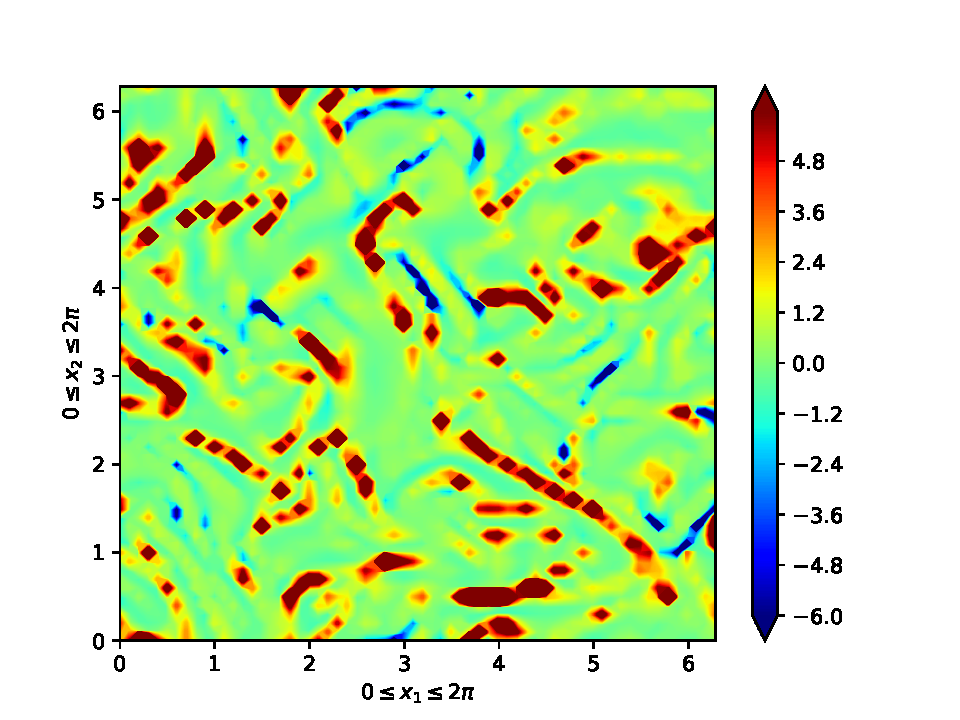
\includegraphics[height=0.4\textheight]{media/run-cds-00/SGS-transport-term-enstrophy}
    \caption{$\Pi_{\Omega}$ results at $z=32$}
\end{figure}

\begin{figure}[H]
    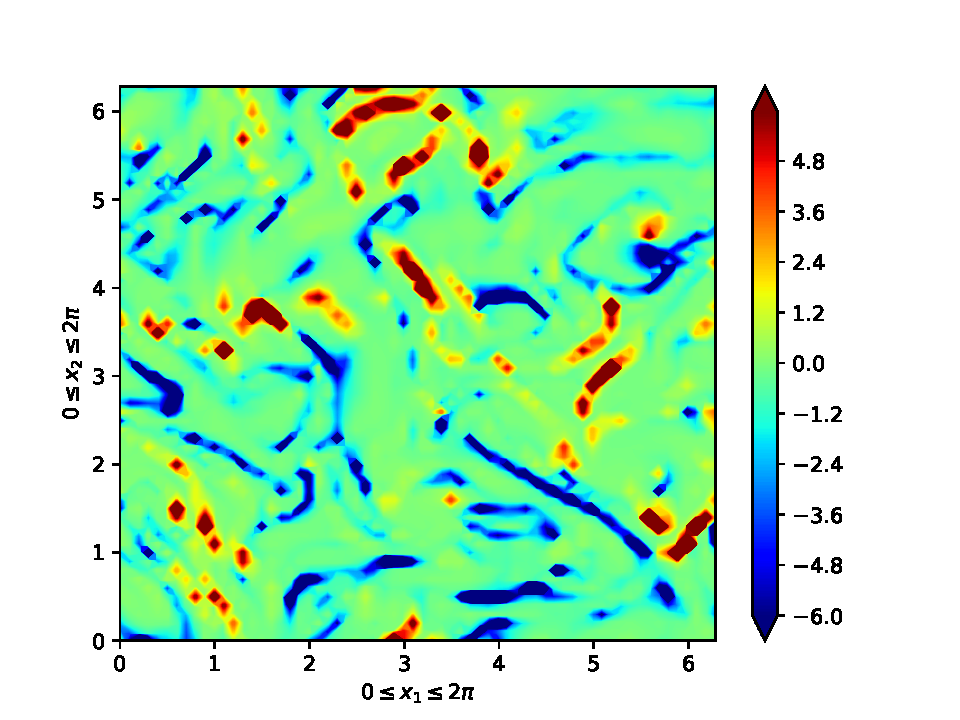
\includegraphics[height=0.4\textheight]{media/run-cds-00/SGS-production-term-enstrophy}
    \caption{$P_{\Omega}$ results at $z=32$}
\end{figure}


